\documentclass[aspectratio=169,11pt]{beamer}

\usepackage[utf8]{inputenc}
\usepackage[T1]{fontenc}
\usepackage[english]{babel}
\usepackage{lmodern}
\usepackage{tikz}
\usetikzlibrary{positioning,arrows.meta}
\usepackage{booktabs}
\usepackage{hyperref}
\usepackage{graphicx}

\definecolor{space}{HTML}{07111F}
\definecolor{panel}{HTML}{101F33}
\definecolor{cyan}{HTML}{57D8E8}
\definecolor{muted}{HTML}{A9B8CC}
\definecolor{warm}{HTML}{FFB86B}

\usetheme{default}
\setbeamercolor{normal text}{fg=white,bg=space}
\setbeamercolor{structure}{fg=cyan}
\setbeamercolor{frametitle}{fg=white,bg=space}
\setbeamercolor{title}{fg=white}
\setbeamercolor{itemize item}{fg=cyan}
\setbeamercolor{itemize subitem}{fg=warm}
\setbeamercolor{block title}{fg=cyan,bg=panel}
\setbeamercolor{block body}{fg=white,bg=panel}
\setbeamertemplate{navigation symbols}{}
\setbeamertemplate{footline}{
  \hfill\color{muted}\insertframenumber\,/\,\inserttotalframenumber
  \hspace{0.6cm}\vspace{0.25cm}
}
\setbeamersize{text margin left=0.8cm,text margin right=0.8cm}
\hypersetup{colorlinks=true,urlcolor=cyan}

\newcommand{\tagline}[1]{{\small\color{muted}#1}}
\newcommand{\keyterm}[1]{{\color{cyan}\textbf{#1}}}
\newcommand{\planet}[3]{%
  \fill[#1] (#2,#3) circle (0.12);
}

\title{The Lost Explorer}
\subtitle{The missions have ended. Their stories live on.}
\author{}
\date{}

\begin{document}


% 1 — Cover
\begin{frame}[plain]
  \begin{tikzpicture}[remember picture,overlay]
    % Imagen de fondo ajustada al tamaño de la diapositiva
    \node[at=(current page.center), inner sep=0pt] {
      \includegraphics[width=\paperwidth, height=\paperheight]{portada-espacial.png}
    };
    % Capa oscura semitransparente para mantener la legibilidad del texto
    \fill[space, opacity=0.65] (current page.south west) rectangle (current page.north east);
  \end{tikzpicture}
  \vspace{0.8cm}
  {\color{cyan}\small NASA SPACE APPS CHALLENGE}\\[0.35cm]
  {\usebeamerfont{title}\Huge\bfseries THE LOST\\EXPLORER}\\[0.35cm]
  {\Large\color{muted}The missions have ended.\\Their stories live on.}\\[0.75cm]
  \tagline{An interactive web experience to explore worlds and space missions.}
\end{frame}

% 2 — Idea
\begin{frame}{The idea: turning space data into exploration}
  \begin{columns}[T,onlytextwidth]
    \column{0.53\textwidth}
      \begin{block}{The starting point}
        Many missions have already concluded, yet their discoveries and adventures
        remain a powerful way to learn about other worlds.
      \end{block}
      \vspace{0.25cm}
      \begin{block}{The proposal}
        A guided tour through the Solar System combining 3D scenes,
        mission stories, and a virtual guide named NOVA.
      \end{block}
    \column{0.42\textwidth}
      \centering
      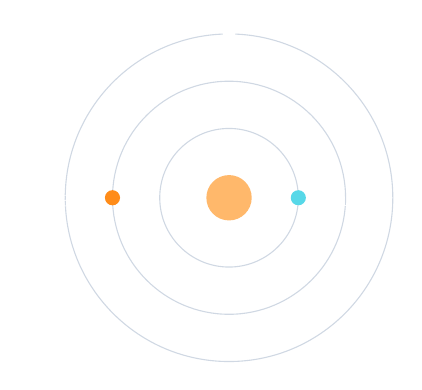
\begin{tikzpicture}[scale=0.8]
        \fill[warm] (0,0) circle (0.36) node[below=0.48cm,text=white] {\small Sun};
        \draw[muted!55] (0,0) circle (1.1);
        \draw[muted!55] (0,0) circle (1.85);
        \draw[muted!55] (0,0) circle (2.6);
        \fill[cyan] (1.1,0) circle (0.12) node[right=0.12cm,text=white] {\small Earth};
        \fill[orange!90] (-1.85,0) circle (0.12) node[left=0.12cm,text=white] {\small Mars};
        \fill[white] (0,2.6) circle (0.10);
      \end{tikzpicture}
      \vspace{0.1cm}

      \tagline{Explore \(\rightarrow\) discover \(\rightarrow\) learn}
  \end{columns}
\end{frame}

% 3 — Experience
\begin{frame}{An interactive journey, from orbit to the surface}
  \begin{columns}[T,onlytextwidth]
    \column{0.32\textwidth}
      \begin{block}{01 \quad Explore}
        Navigate a 3D representation of the Solar System and choose a destination.
      \end{block}
    \column{0.32\textwidth}
      \begin{block}{02 \quad Discover}
        Visit Apollo lunar sites or learn about nine missions that reached Mars.
      \end{block}
    \column{0.32\textwidth}
      \begin{block}{03 \quad Interact}
        Examine surface scenes and selected rover models.
      \end{block}
  \end{columns}
  \vspace{0.3cm}
  \begin{alertblock}{Guidance}
    NOVA provides contextual messages and animations throughout the experience;
    controls support mouse, touchscreen, and on-screen controls.
  \end{alertblock}
\end{frame}

% 4 — Stories
\begin{frame}{The missions: science told through its milestones}
  \begin{columns}[T,onlytextwidth]
    \column{0.53\textwidth}
      \begin{itemize}
        \item \keyterm{Sojourner (1997):} first rover demonstration on Mars; operated for 83 days.
        \item \keyterm{Spirit (2004):} a wheel exposed silica-rich soil in Gusev crater.
        \item \keyterm{Opportunity (2004):} traveled 45.16 km and found evidence of past water.
        \item \keyterm{Curiosity (2012) and Perseverance (2021):} study environments and samples in Gale and Jezero.
      \end{itemize}
    \column{0.42\textwidth}
      \begin{block}{More than a timeline}
        Each mission is presented through its exploration site, its objective,
        notable instruments or findings, and, when available,
        a 3D model.
      \end{block}
      \vspace{0.2cm}
      \tagline{Also includes Viking 1 and 2, Phoenix, and InSight.}
  \end{columns}
\end{frame}

% 5 — Technology
\begin{frame}{How the experience is built}
  \centering
  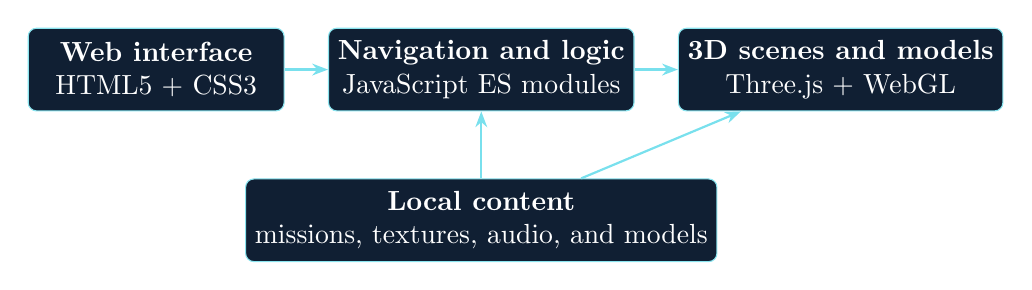
\begin{tikzpicture}[
    node distance=0.55cm,
    box/.style={draw=cyan!70,rounded corners=3pt,fill=panel,
                minimum width=3.25cm,minimum height=1.05cm,
                align=center,text=white},
    link/.style={-{Stealth[length=2mm]},draw=cyan!80,line width=0.8pt}
  ]
    \node[box] (ui) {\textbf{Web interface}\\HTML5 + CSS3};
    \node[box,right=of ui] (app) {\textbf{Navigation and logic}\\JavaScript ES modules};
    \node[box,right=of app] (scene) {\textbf{3D scenes and models}\\Three.js + WebGL};
    \node[box,below=0.85cm of app] (assets) {\textbf{Local content}\\missions, textures, audio, and models};
    \draw[link] (ui) -- (app);
    \draw[link] (app) -- (scene);
    \draw[link] (assets) -- (app);
    \draw[link] (assets) -- (scene);
  \end{tikzpicture}
  \vspace{0.45cm}
  \begin{block}{Development}
    Vite serves the application during development and generates the production
    build. The experience runs in the browser and requires
    WebGL support for the 3D scenes.
  \end{block}
\end{frame}

% 6 — Design
\begin{frame}{Designed to discover at your own pace}
  \begin{columns}[T,onlytextwidth]
    \column{0.48\textwidth}
      \begin{block}{Interaction}
        \begin{itemize}
          \item Rotate scenes by dragging; zoom in or out.
          \item Use touch gestures on compatible devices.
          \item Follow links to NASA mission pages.
        \end{itemize}
      \end{block}
    \column{0.48\textwidth}
      \begin{block}{Experience criteria}
        \begin{itemize}
          \item NOVA guides without replacing exploration.
          \item Stories connect places, artifacts, and findings.
          \item Reduced-motion preferences are respected in supported transitions.
        \end{itemize}
      \end{block}
  \end{columns}
  \vspace{0.25cm}
  \centering
  {\large\color{cyan}\textbf{An invitation to explore the science behind every mission.}}
\end{frame}

% 7 — Sources and closing
\begin{frame}{Sources and closing}
  \begin{columns}[T,onlytextwidth]
    \column{0.56\textwidth}
      \textbf{\color{cyan}Content sources}
      \begin{itemize}
        \item Project: README and mission data from The Lost Explorer.
        \item NASA Science: \href{https://science.nasa.gov/mission/mars-pathfinder/}{Mars Pathfinder},
          \href{https://science.nasa.gov/mission/mer-spirit/}{Spirit},
          \href{https://science.nasa.gov/mission/mer-opportunity/}{Opportunity}.
        \item NASA Science: \href{https://science.nasa.gov/mission/mars-2020-perseverance/}{Perseverance},
          \href{https://science.nasa.gov/mission/msl-curiosity/}{Curiosity}.
      \end{itemize}
      \vspace{0.15cm}
      \tagline{More mission references: NASA Science.}
    \column{0.39\textwidth}
      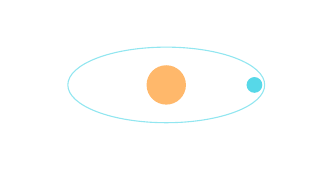
\begin{tikzpicture}
        \fill[warm] (0,0) circle (0.25);
        \draw[cyan!65] (0,0) ellipse (1.25 and 0.48);
        \fill[cyan] (1.12,0) circle (0.10);
        \draw[white!35] (0,0) ellipse (1.75 and 0.72);
        \fill[white] (-1.68,0.12) circle (0.08);
      \end{tikzpicture}
      \vspace{0.35cm}

      {\Large\bfseries Let the exploration begin!}\\[0.15cm]
      \tagline{The Lost Explorer}
  \end{columns}
\end{frame}

\end{document}
